%narms.tex, an example driver file for Balkema documents.

%use the following for A4 paper:
\documentclass[12pt,a4paper,twocolumn,fleqn]{narms}

% packages needed
\usepackage{subfigure}
\usepackage{epsfig}
\usepackage{timesmt}

% add here more packages based on the document format


% setting math equation indent from left 0pts

\mathindent=0pt%

% use this for chicaco style reference
% Author references
% IMPORTANT: Author wants to format references in chicaco style Author must use BiBTex
% IMPORTANT: Author wants to format numbered references remove chicaco style file and \bibliographystyle{chicaco}

\usepackage{chicaco}

%  \cite{key}
%    which produces citations with full author list and year.
%    eg. (Brown 1978; Jarke, Turner, Stohl, et al. 1985)

%  \citeNP{key}
%    which produces citations with full author list and year, but without
%    enclosing parentheses:
%    eg. Brown 1978; Jarke, Turner & Stohl 1985

%  \citeA{key}
%    which produces citations with only the full author list.
%    eg. (Brown; Jarke, Turner & Stohl)

%  \citeANP{key}
%    which produces citations with only the full author list, without
%    parentheses eg. Brown; Jarke, Turner & Stohl

%  \citeN{key}
%    which produces citations with the full author list and year, but
%    can be used as nouns in a sentence; no parentheses appear around
%    the author names, but only around the year.
%      eg. Shneiderman (1978) states that......
%    \citeN should only be used for a single citation.

%  \shortcite{key}
%    which produces citations with abbreviated author list and year.

%  \shortciteNP{key}
%    which produces citations with abbreviated author list and year.

%  \shortciteA{key}
%    which produces only the abbreviated author list.

%  \shortciteANP{key}
%    which produces only the abbreviated author list.

%  \shortciteN{key}
%    which produces the abbreviated author list and year, with only the
%    year in parentheses. Use with only one citation.

%  \citeyear{key}
%    which produces the year information only, within parentheses.

%  \citeyearNP{key}
%    which produces the year information only.


%%%%%%%%%%%%%%%%%%%%%%%%%%%%%%%%%%%%%%%%%%%%%%%%%%%%%%%%%%%%%%%%%%%
%%%  All this stuff is from modifying the article.cls for Balkema
%%%  specifications.

%\title{...}
%\author{...}
%use \aff for author affiliations
% use \authornext for from second author
% empty line space between multiple authors
%\abstract{...}
%\maketitle{}

%%%%%%% Style for TABLES
% insert tabular command inside \tabletext{} this will produce tables in 10pts

\begin{document}
\title{Fast early flood warning systems exploiting catchment specific behavior}
\author{{S. Rusca} \\
{\aff{ETH Zurich, Switzerland}} \\\\
{\authornext{J. P. Carbajal}}\\
{\aff{University of ???}}
%{\authornext{R. Schielen}}\\
%{\aff{Department of Water Engineering and Management}} \\
%{\aff{University of Twente, Enschede, The Netherlands.}}\\
} \maketitle


\section*{Abstract}

Floods due to heavy rain are among the most destructive events in hydrology. 
Numerical models cannot directly be used for real time flood prediction due to
their high complexity. Ad hoc surrogate models provide great speed
ups with minor accuracy losses.


\section{Introduction}

{\bf The text in this paper is for visual purpose only. No rights
can be taken from this.}\\

The submission of Extended Abstract to $5^{th}$ IAHR Europe Congress
is available on the website of the congress at: http://events.unitn.it/en/iahr2018.\\

Follow the instructions.\\

Here some lines as example of the template of the Extended Abstract.\\

A detailed riparian field study to assess the im-portance of
bedrock groundwater in streamflow processes was established in the
headwaters of the Afon Hafren, mid-Wales, UK. Results from this
study identified distinct groundwater horizons close to the stream
channel.  Different flow pathways and travel times resulted in a
different chemical charac-ter of groundwaters in these different
horizons.  Groundwater discharge from these horizons into the
stream was by piston displacement in response to re-charging
rainfall higher up in the catchment.  Groundwater upwelling into
the soils indicated soil water to be sourced from both groundwater
and rain-fall.  Soil waters closest to the stream (ca. 25m) were
predominantly groundwater controlled and may be the major source
for ecologically toxic soil compo-nents such as aluminium entering
the river.

A detailed riparian field study to assess the im-portance of
bedrock groundwater in streamflow processes was established in the
headwaters of the Afon Hafren, mid-Wales, UK.  Results from this
study identified distinct groundwater horizons close to the stream
channel.  Different flow pathways and travel times resulted in a
different chemical charac-ter of groundwaters in these different
horizons.


\begin{figure}[h!]
\centerline{
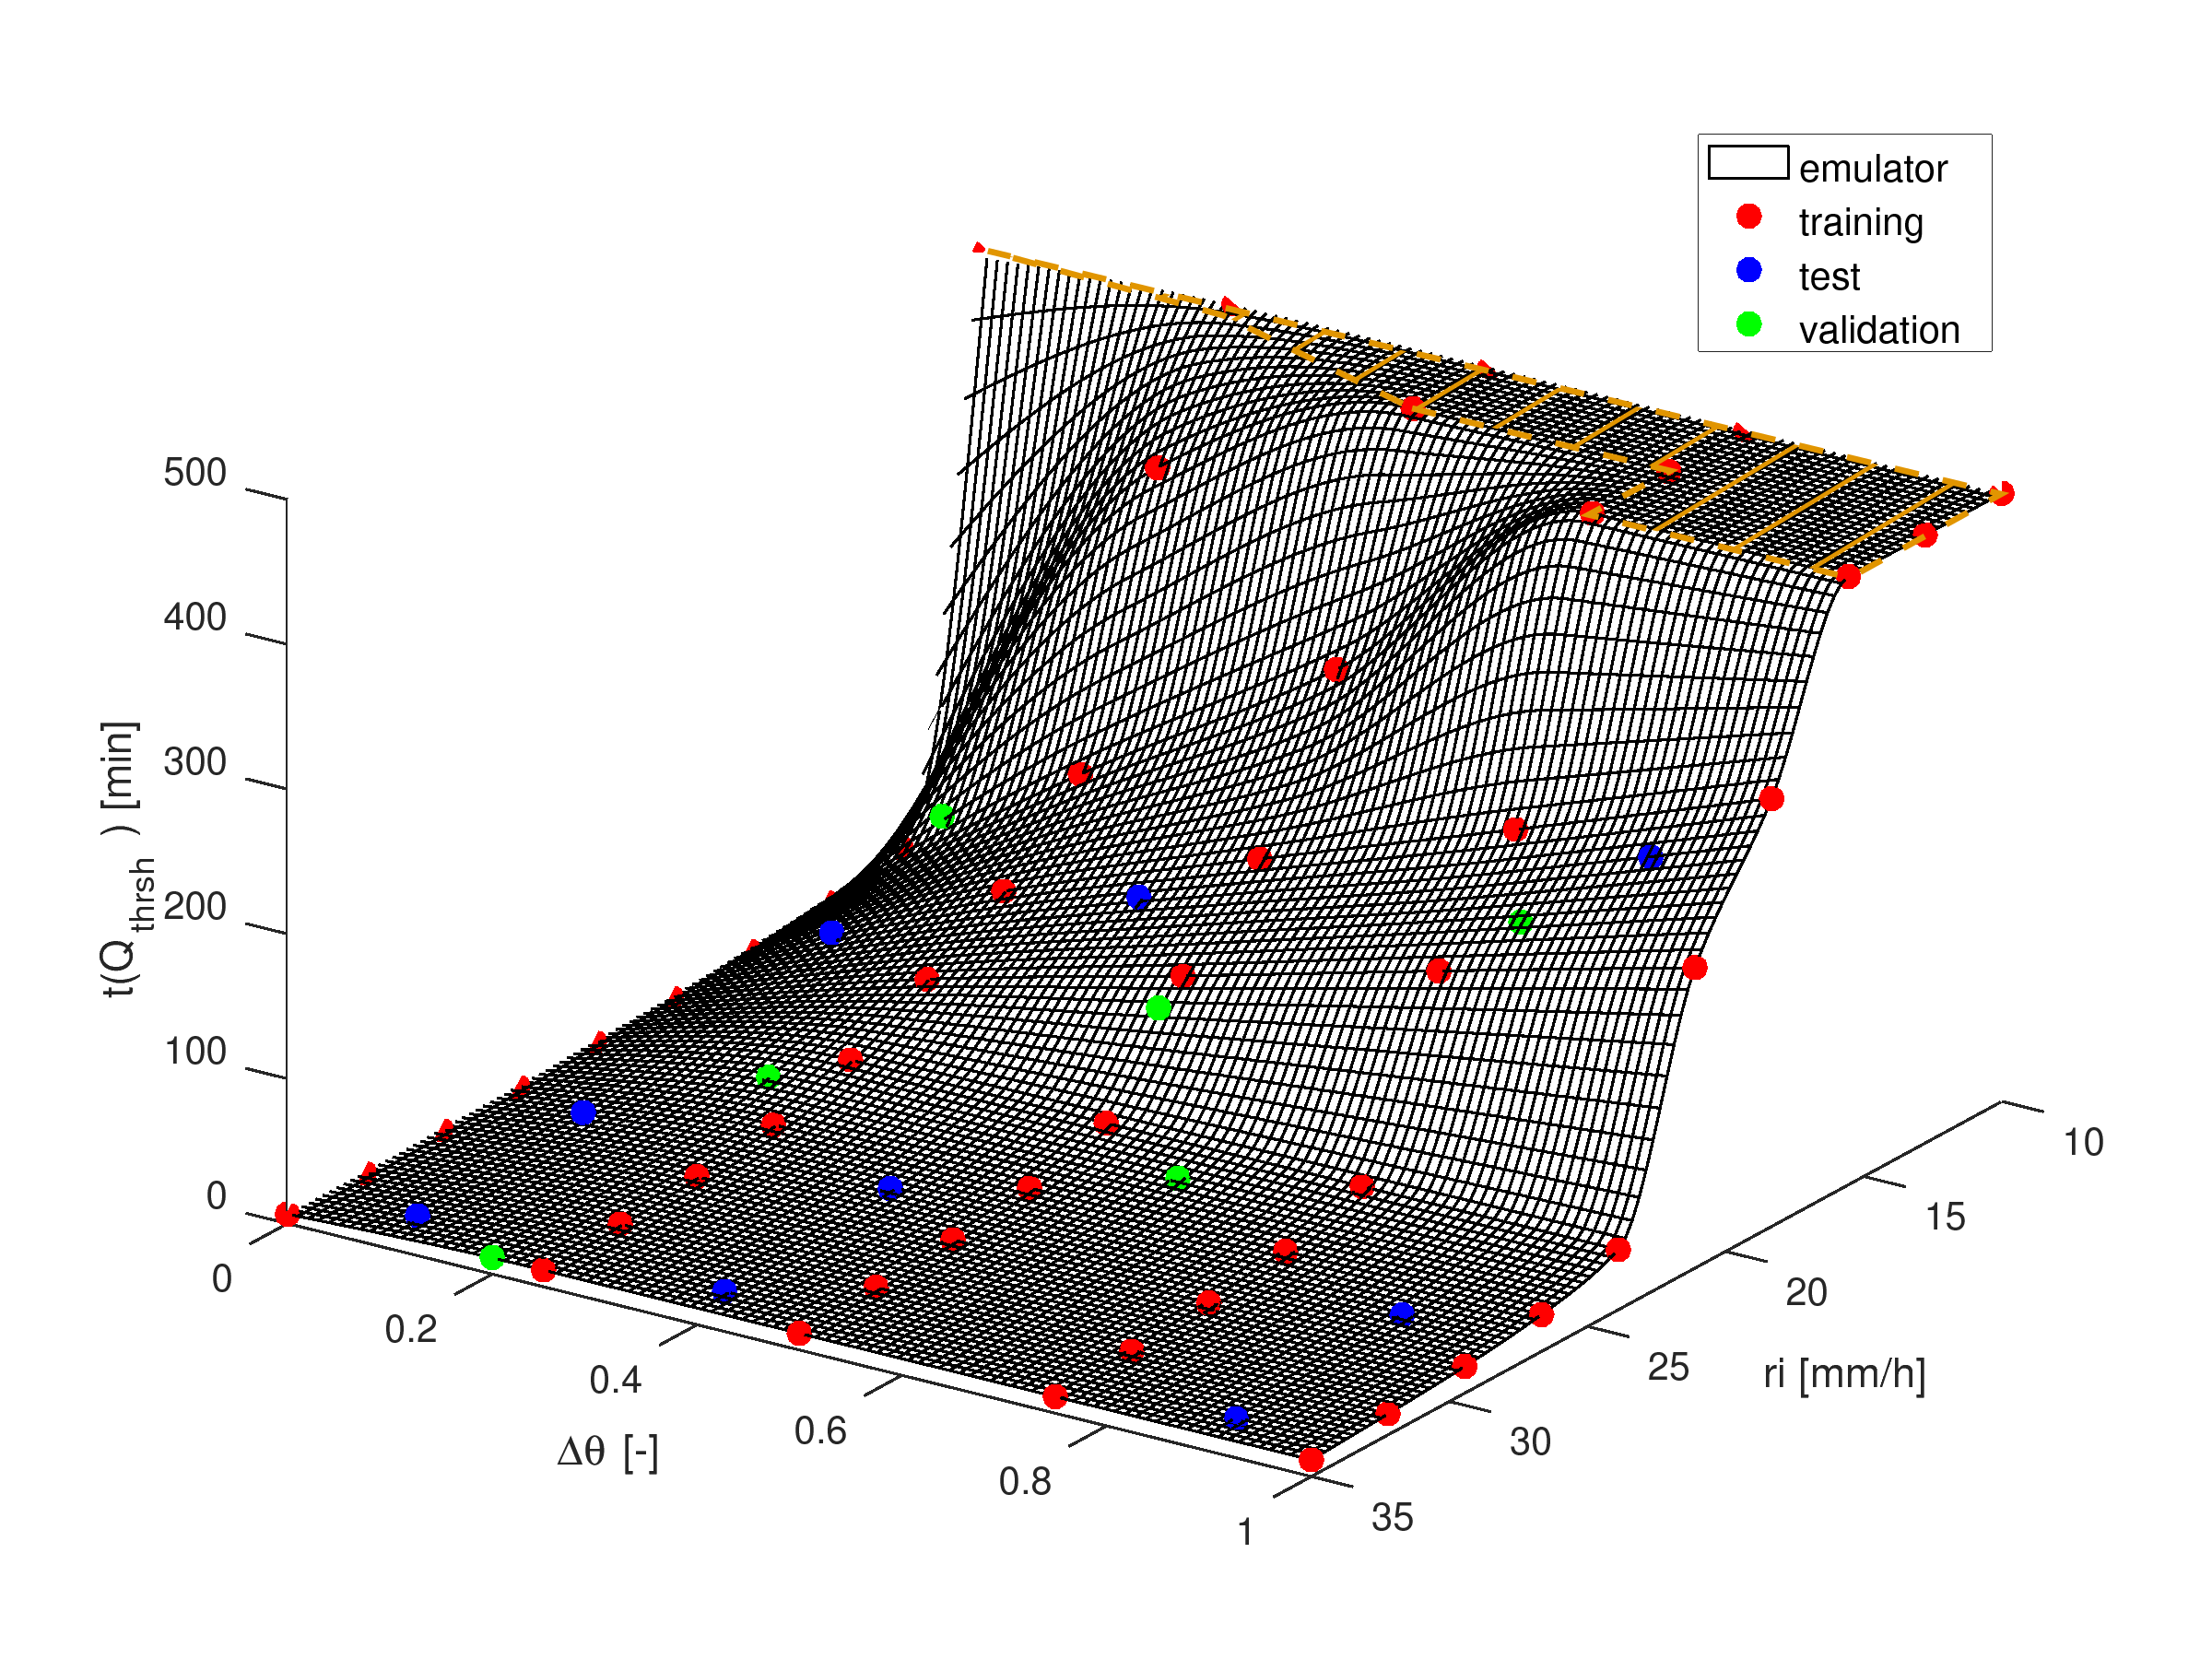
\includegraphics[width=8cm]{img/emulator.png}
} \caption{Sketch of flow configuration} \label{f:sketch1}
\end{figure}


A detailed riparian field study to assess the im-portance of
bedrock groundwater in streamflow processes was established in the
headwaters of the Afon Hafren, mid-Wales, UK.  Results from this
study identified distinct groundwater horizons close to the stream
channel.


\begin{table}
\caption{Margin settings for A4 size paper and letter size paper.}
\tabletext{
\begin{tabular}{lllll}\hline
&\multicolumn{2}{l}{A4 size
paper}&\multicolumn{2}{l}{Letter size paper}\\[-6pt]
&\multicolumn{2}{l}{\hrulefill}&\multicolumn{2}{l}{\hrulefill}\\
Setting&cm&inches&cm&inches\\\hline
Top&1.2&0.47"&0.32&0.13"\\
Bottom&1.3&0.51"&0.42&0.17"\\
Left&1.15&0.45"&1.45&0.57"\\
Right&1.15&0.45"&1.45&0.57"\\
All other&0.0&0.0"&0.0&0.0"\\
Column width*&9.0&3.54"&9.0&3.54"\\
Column spacing*&0.7&0.28"&0.7&0.28"\\\hline
\end{tabular}}
\end{table}

\subsection{Equation}

You can add an equation:

\begin{equation}\label{eqn}
  a=1
\end{equation}
and refer to eq.(\ref{eqn}).

\section{Acknowledge}

Here you can insert acknowledge.

\bibliography{ref}
\bibliographystyle{chicaco}



\end{document}
